\section{Aufbau}
\label{sec:Aufbau}
In Abbildung \ref{fig:Versuchsaufbau} ist der Versuchsaufbau zu sehen.

    \begin{figure}[H]
        \centering
        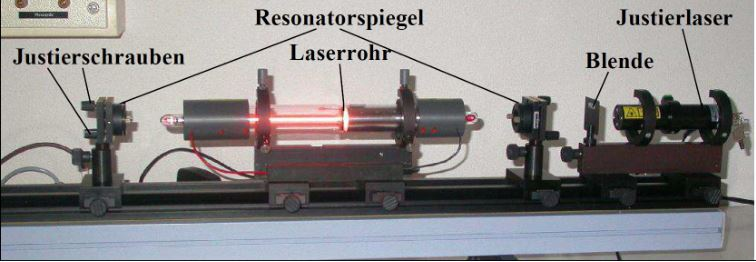
\includegraphics[width=1\textwidth]{images/HeNeAufbau.JPG}
        \caption{Versuchsaufbau. \cite{V61}}
        \label{fig:Versuchsaufbau}
    \end{figure}

\noindent
In der Abbildung ist rechts der zur Justage nötige Justierlaser ($\lambda = \SI{532}{\nano\metre}$, 
$P_\text{max} = \SI{1}{\milli\watt}$, $P_\text{grün} = \SI{0.2}{\milli\watt}$) zu sehen.    
An den Enden des Laserrohrs befinden sich sogenannte Brewster-Fenster, die dafür sorgen, dass das Laserlicht eine definierte Polarisationsrichtung erhält. Die bei den anschließenden Messungen notwendigen Komponenten, wie eine Photodiode oder ein Polarisationsfilter, werden jeweils auf der Schiene, auf der sich der Laser befindet, beweglich angeordnet.

\section{Durchführung}
\label{sec:Durchführung}
Zu Beginn des Versuchs muss der Aufbau mit Hilfe des Justierlasers justiert werden. Dazu werden die Spiegel so ausgerichtet, dass die Reflexe beider Spiegel auf das Fadenkreuz auf der Justierblende treffen. Falls keine Lasertätigkeit einsetzt, müssen die Resonatorspiegel sehr vorsichtig nachjustiert werden. Im Anschluss werden verschiedene Messungen mit dem justierten Versuchsaufbau durchgeführt.

\subsection{Untersuchung der $TEM$-Moden}

Für die Untersuchung der $TEM$-Moden wird ein dünner Wolframdraht (Dicke $d = \SI{0.005}{\milli\metre}$) zwischen den Laser und die Resonatorspiegel
gestellt. Durch die Zerstreuung des Laserstrahls mit einer Zerstreulinse können dann verschiedene Moden auf der hinteren Projektionsfläche beobachtet werden. Die Lichtintensität wird dann mittels einer Photodiode gemessen, welche per Schraube fein verstellt werden kann.

\subsection{Überprüfen der Stabilitätsbedingung}
Für das Überprüfen der Stabilitätsbedingung in Abhängigkeit von der Resonatorlänge wird die Resonatorlänge in kleinen Schritten erhöht bis die maximal mögliche Resonatorlänge erreicht ist. Dabei kann es passieren, dass die Lasertätigkeit beim Verstellen der Spiegel abbricht. Dann muss der Versuchsaufbau fein nachjustiert werden bis die Lasertätigkeit wieder einsetzt. Die Überprüfung der Stabilitätsbedingung wird für zwei unterschiedliche Resonatoren durchgeführt. Einmal für einen Resonator mit zwei konkaven Spiegeln und einmal für einen Resonator mit einem konkaven und einem planparallelen Spiegel.

\subsection{Untersuchung von Multimodenbetrieb und Frequenzspektrum}
Es werden die Schwebungsfrequenzen mithilfe einer schnellen Photodiode (Bandbreite bis $\SI{1}{\giga\hertz}$) vermessen. An diese wird ein Oszilloskop als Spektrumanalysator angeschlossen, um die Fourierspektren für unterschiedliche Resonatorlängen $L$ zu messen.

\subsection{Bestimmung der Polarisation}
Zur Bestimmung der Polarisation wird ein Polarisationsfilter in den Strahlengang gestellt. Mit dem Polarisationsfilter wird die Polarisationsrichtung in $\SI{10}{\degree}$ Schritten verändert. Gemessen und notiert wird dann die Lichtintensität in Abhängigkeit von der Polarisation.

\subsection{Bestimmung der Wellenlänge}
Für die Bestimmung der Wellenlänge werden 4 unterschiedliche Gitter mit verschiedenen Gitterkonstanten in den Strahlengang gestellt, sodass jeweils ein Interferenzmuster entsteht. Anschließend wird der Abstand zwischen den Beugungsmaxima mit einem Maßband vermessen und notiert.